
%(BEGIN_QUESTION)
% Copyright 2010, Tony R. Kuphaldt, released under the Creative Commons Attribution License (v 1.0)
% This means you may do almost anything with this work of mine, so long as you give me proper credit

Acetone -- a valuable industrial solvent (chemical formula C$_{3}$H$_{6}$O) -- may be manufactured from isopropyl alcohol (chemical formula C$_{3}$H$_{8}$O) in a chemical reaction that breaks two atoms of hydrogen away from each molecule of alcohol, leaving acetone and hydrogen gas (H$_{2}$) as byproducts:

$$\hbox{C}_3\hbox{H}_8\hbox{O} \rightarrow \hbox{C}_3\hbox{H}_6\hbox{O} + \hbox{H}_2$$

A simplified flow diagram for this process is shown here:

$$\includegraphics[width=15.5cm]{i00912x01.eps}$$

Supposing each of the labeled flowmeters registers {\it true mass flow} rather than volumetric flow, determine the flow rates that should be shown by FT-2 and FT-6, based on the other mass flow rates shown in the system.  Assume perfect mass balance in this process (i.e. no leaks, fugitive emissions, etc.).

\vskip 10pt

FT-2 = \underbar{\hskip 50pt} kg/min

\vskip 10pt

FT-6 = \underbar{\hskip 50pt} kg/min

\underbar{file i00912}
%(END_QUESTION)





%(BEGIN_ANSWER)

5 points for each answer:

\vskip 10pt

FT-2 = \underbar{\bf 10.4} kg/min

\vskip 10pt

FT-6 = \underbar{\bf 0.9} kg/min

%(END_ANSWER)





%(BEGIN_NOTES)

{\bf This question is intended for exams only and not worksheets!}.

%(END_NOTES)


